The Component Diagram shown below describes the logical components of the system we are to develop, from a very high-level description on to a more detailed one. This diagram does not take into account the deployment phase, hence it doesn't describe the logical layer of the system in terms of the physical tiers where it is deployed. It also does not show the interfaces between the logical layer and the end users or the database, for simplicity %TODO do we have to add them?

	\subsubsection{High level components}
		\paragraph{} We shall show below the high level view of the logical components of the system and their interactions. Following the UML 1 notation, the dashed arrows represent dependencies between components, with the tail end component depending on the point end component (e.g. if \textit{A -> B}, then A \textit{depends on} B). 

		
		\begin{figure}[h]
			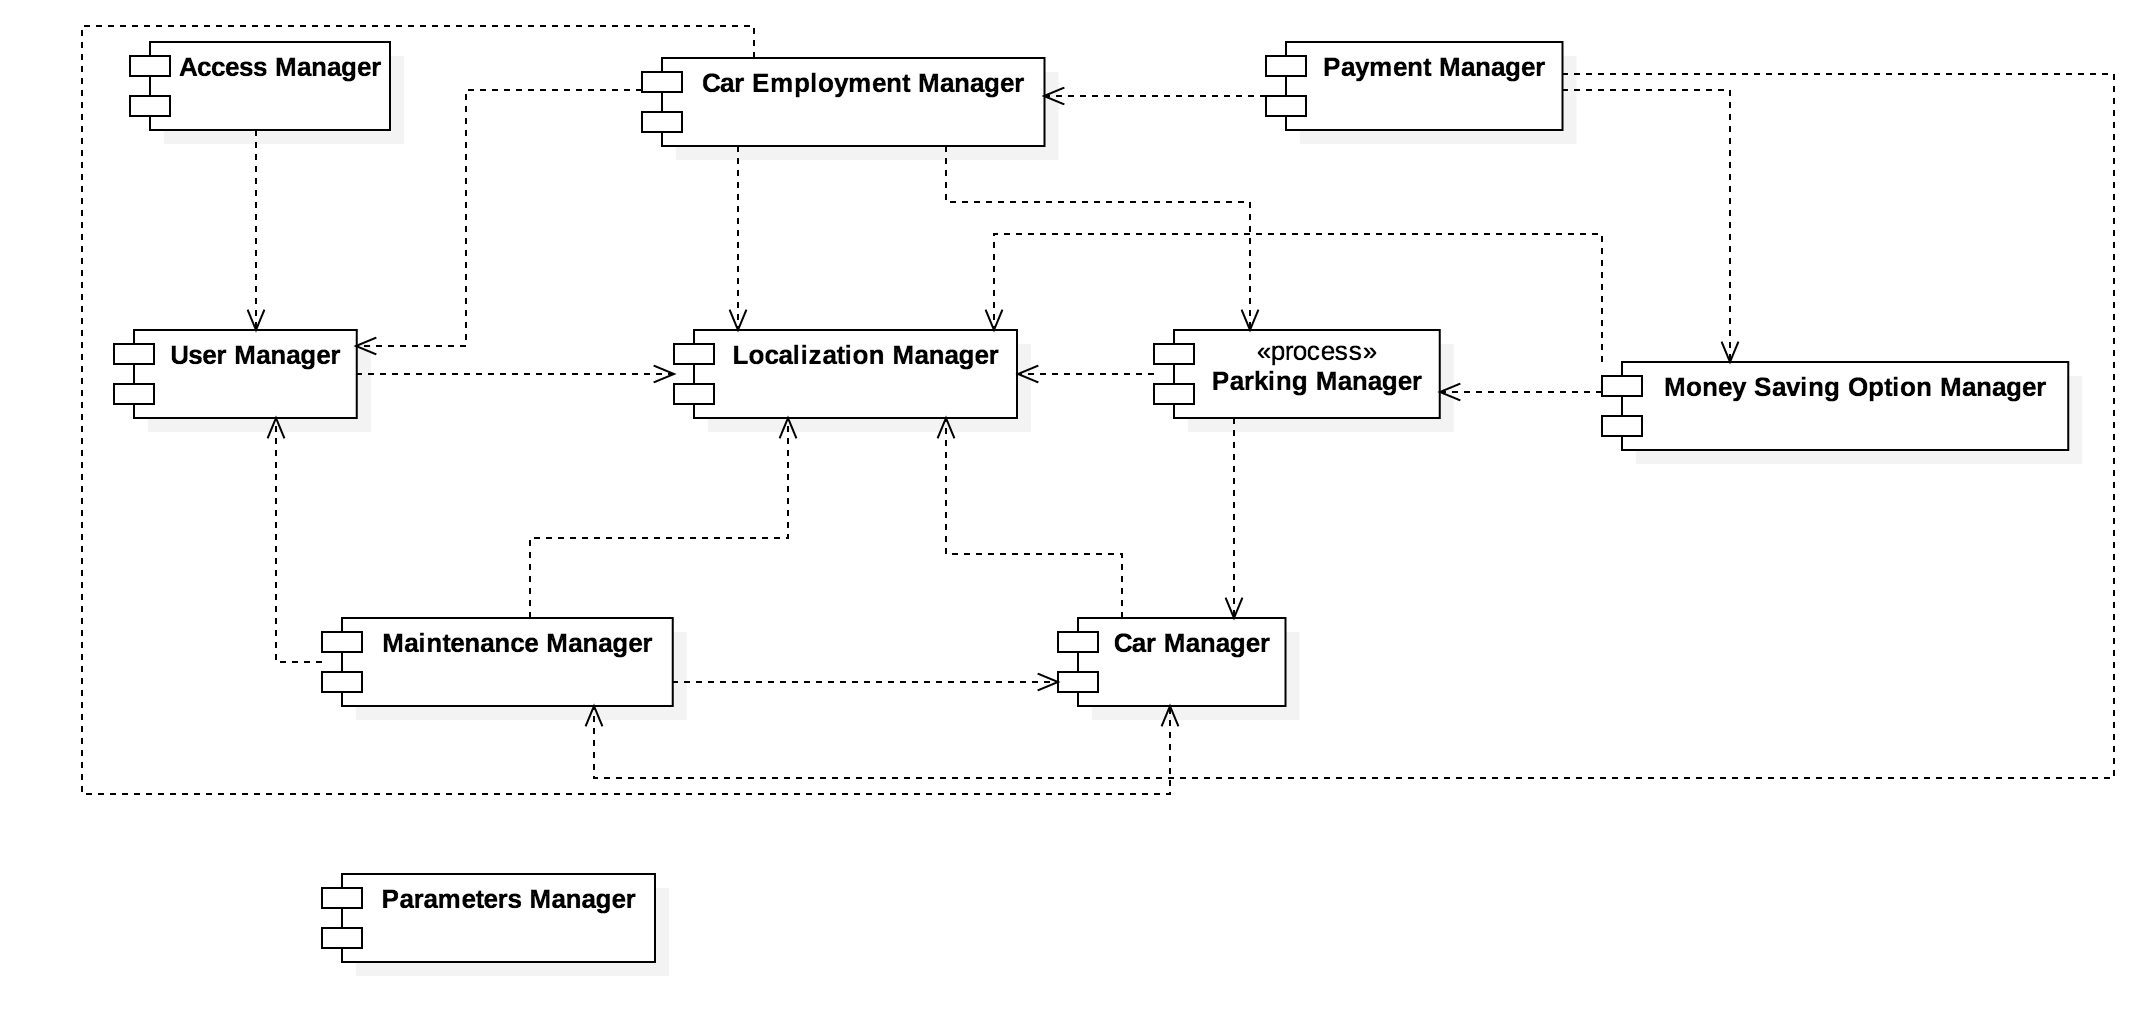
\includegraphics[scale=0.24]{img/component_diagrams/01_high_level_component_view.png}
		\end{figure}

	\subsubsection{Component view}
	
	
	
		\paragraph{Access Manager}
		
			\begin{figure}[h]
				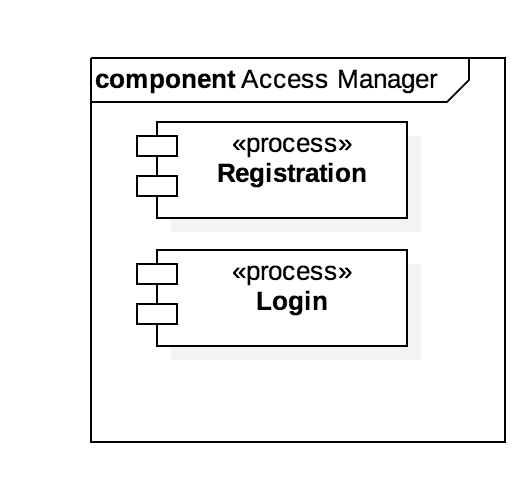
\includegraphics[scale=0.4, center]{img/component_diagrams/02_access_manager.png}
			\end{figure}
			
		\paragraph{}The Access Manager deals with the first interactions of a user or a guest with the system at the beginning of each session. Every further interaction with the system requires either a log in or the registration, both of which are managed by independent processes. The login interfaces with the User Handler to verify the validity of the login information and to allow the authenticated user to continue employing the system. Both processes also interface with the database.
		
		
		
		
		\paragraph{User Manager}
		
			\begin{figure}[h]
				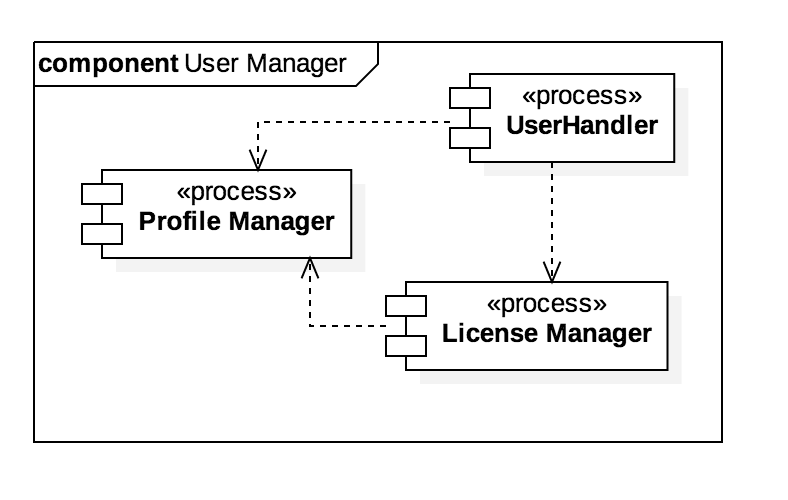
\includegraphics[scale=0.4, center]{img/component_diagrams/03_user_manager.png}
			\end{figure}
			
		\paragraph{}